\chapter{Integration schemes}

\section{First order integrators for the harmonic oscillator}

\begin{sourcefiles}
  \item[Source code] src/091\_first\_order.c
  \item[Analysis script] src/091\_first\_order.R
  \item[Executable] src/091\_first\_order
\end{sourcefiles}

The Hamilton’s equations of motion for the one-dimensional harmonic oscillator
are:
\begin{equation}
  \begin{dcases}
    \dot{p} = \pdiff{\mathcal{H}}{x} = - kx, \\
    \dot{x} = \pdiff{\mathcal{H}}{p} = \frac{p}{m},
  \end{dcases}
\end{equation}
where the Hamiltonian is given by
\begin{equation}
  \mathcal{H} = \frac{p^{2}}{2m} + \frac{kx^{2}}{2}.
  \label{eq:harm-osc-H}
\end{equation}
The exercise asked to compare two integrators, the non-symplectic Euler
integrator:
\begin{equation}
  \begin{cases}
    p_{t + \Delta t} = p_{t} - x_{t} \Delta t, \\
    x_{t + \Delta t} = x_{t} + p_{t} \Delta t,
  \end{cases}
  \label{eq:non-symp}
\end{equation}
and another first order integrator, but symplectic:
\begin{equation}
  \begin{cases}
    p_{t + \Delta t} = p_{t} - x_{t} \Delta t, \\
    x_{t + \Delta t} = x_{t} + p_{t + \Delta t} \Delta t.
  \end{cases}
  \label{eq:symp}
\end{equation}

If we express \cref{eq:non-symp,eq:symp} in matrix form, we get
\begin{align}
  \begin{pmatrix}
    x \\ p  
  \end{pmatrix}_{t + \Delta t}
  &=
  \begin{pmatrix}
    1 & \Delta t \\
    -\Delta t & 1
  \end{pmatrix}
  \begin{pmatrix}
    x \\ p
  \end{pmatrix}_{t}, \\
  \begin{pmatrix}
    x \\ p
  \end{pmatrix}_{t + \Delta t}
  &=
  \begin{pmatrix}
    1 - \Delta t^{2} & \Delta t \\
    - \Delta t & 1
  \end{pmatrix}
  \begin{pmatrix}
    x \\ p
  \end{pmatrix}_{t}.
\end{align}
The determinants of the update matrices are then
\begin{align}
  \det \begin{pmatrix}
    1 & \Delta t \\
    - \Delta t & 1
  \end{pmatrix}
  &= 1 + \Delta t^{2} > 1 \\
  \det \begin{pmatrix}
    1 - \Delta t^{2} & \Delta t \\
    - \Delta t & 1
  \end{pmatrix}
  &= 1 - \Delta t^{2} + \Delta t^{2} = 1.
\end{align}
This means that only the integrator in \cref{eq:symp} preserves the phase space
measure, while the non-symplectic Euler integrator will display an exponentially
growing error in the energy.

Actually, the symplectic integrator in \cref{eq:symp} does not strictly conserve
the Hamiltonian $\mathcal{H}$ in \cref{eq:harm-osc-H}, but a \emph{shadow
Hamiltonian} $\mathcal{H}^{\prime}$. If we set for convenience $k = m = 1$,
$\mathcal{H}^{\prime}$ takes the form
\begin{equation}
  \mathcal{H}^{\prime} = \mathcal{H} - \frac{p x}{2} \Delta t.
  \label{eq:shadow-H}
\end{equation}
Indeed, if we calculate $\mathcal{H}^{\prime}$ at time $t + \Delta t$, following
the transformation, we get
\begin{equation}
  \begin{split}
    \mathcal{H}^{\prime}(x_{t + \Delta t}, p_{t + \Delta t})
    &= \frac{1}{2} (p_{t} - x_{t} \Delta t)^{2} + \frac{1}{2} \bigl[ (1 - \Delta
    t^{2}) x_{t} + p_{t} \Delta t \bigr]^{2} \\
    &\qquad -\frac{\Delta t}{2} (p_{t} - x_{t} \Delta t) \bigl[ (1 - \Delta
    t^{2}) x_{t} + p_{t} \Delta t \bigr] \\
    &= \frac{1}{2} \bigl[
      p_{t}^{2} + \cancel{x_{t}^{2} \Delta t^{2}} - \cancel{2 x_{t} p_{t} \Delta
      t} + x_{t}^{2} + \cancel{x_{t}^{2} \Delta t^{4}} - \cancel{2 x_{t}^{2}
      \Delta t^{2}} + \cancel{p_{t}^{2} \Delta t^{2}} \\
    &\qquad + \cancel{2 x_{t} p_{t} \Delta t} - \cancel{2 x_{t} p_{t} \Delta
    t^{3}} - x_{t} p_{t} \Delta t + \cancel{x_{t} p_{t} \Delta t^{3}} \\
    &\qquad -\cancel{p_{t}^{2} \Delta t^{2}} + \cancel{x_{t}^{2} \Delta t^{2}} -
    \cancel{x_{t}^{2} \Delta t^{4}} + \cancel{x_{t} p_{t} \Delta t^{3}}
    \bigr] \\
    &= \frac{x_{t}^{2} + p_{t}^{2}}{2} - \frac{x_{t} p_{t}}{2} \Delta t \\
    &= \mathcal{H}(x_{t}, p_{t}) - \frac{x_{t} p_{t}}{2} \Delta t \\
    &= \mathcal{H}^{\prime}(x_{t}, p_{t}).
  \end{split}
\end{equation}

\begin{figure}
  \centering
  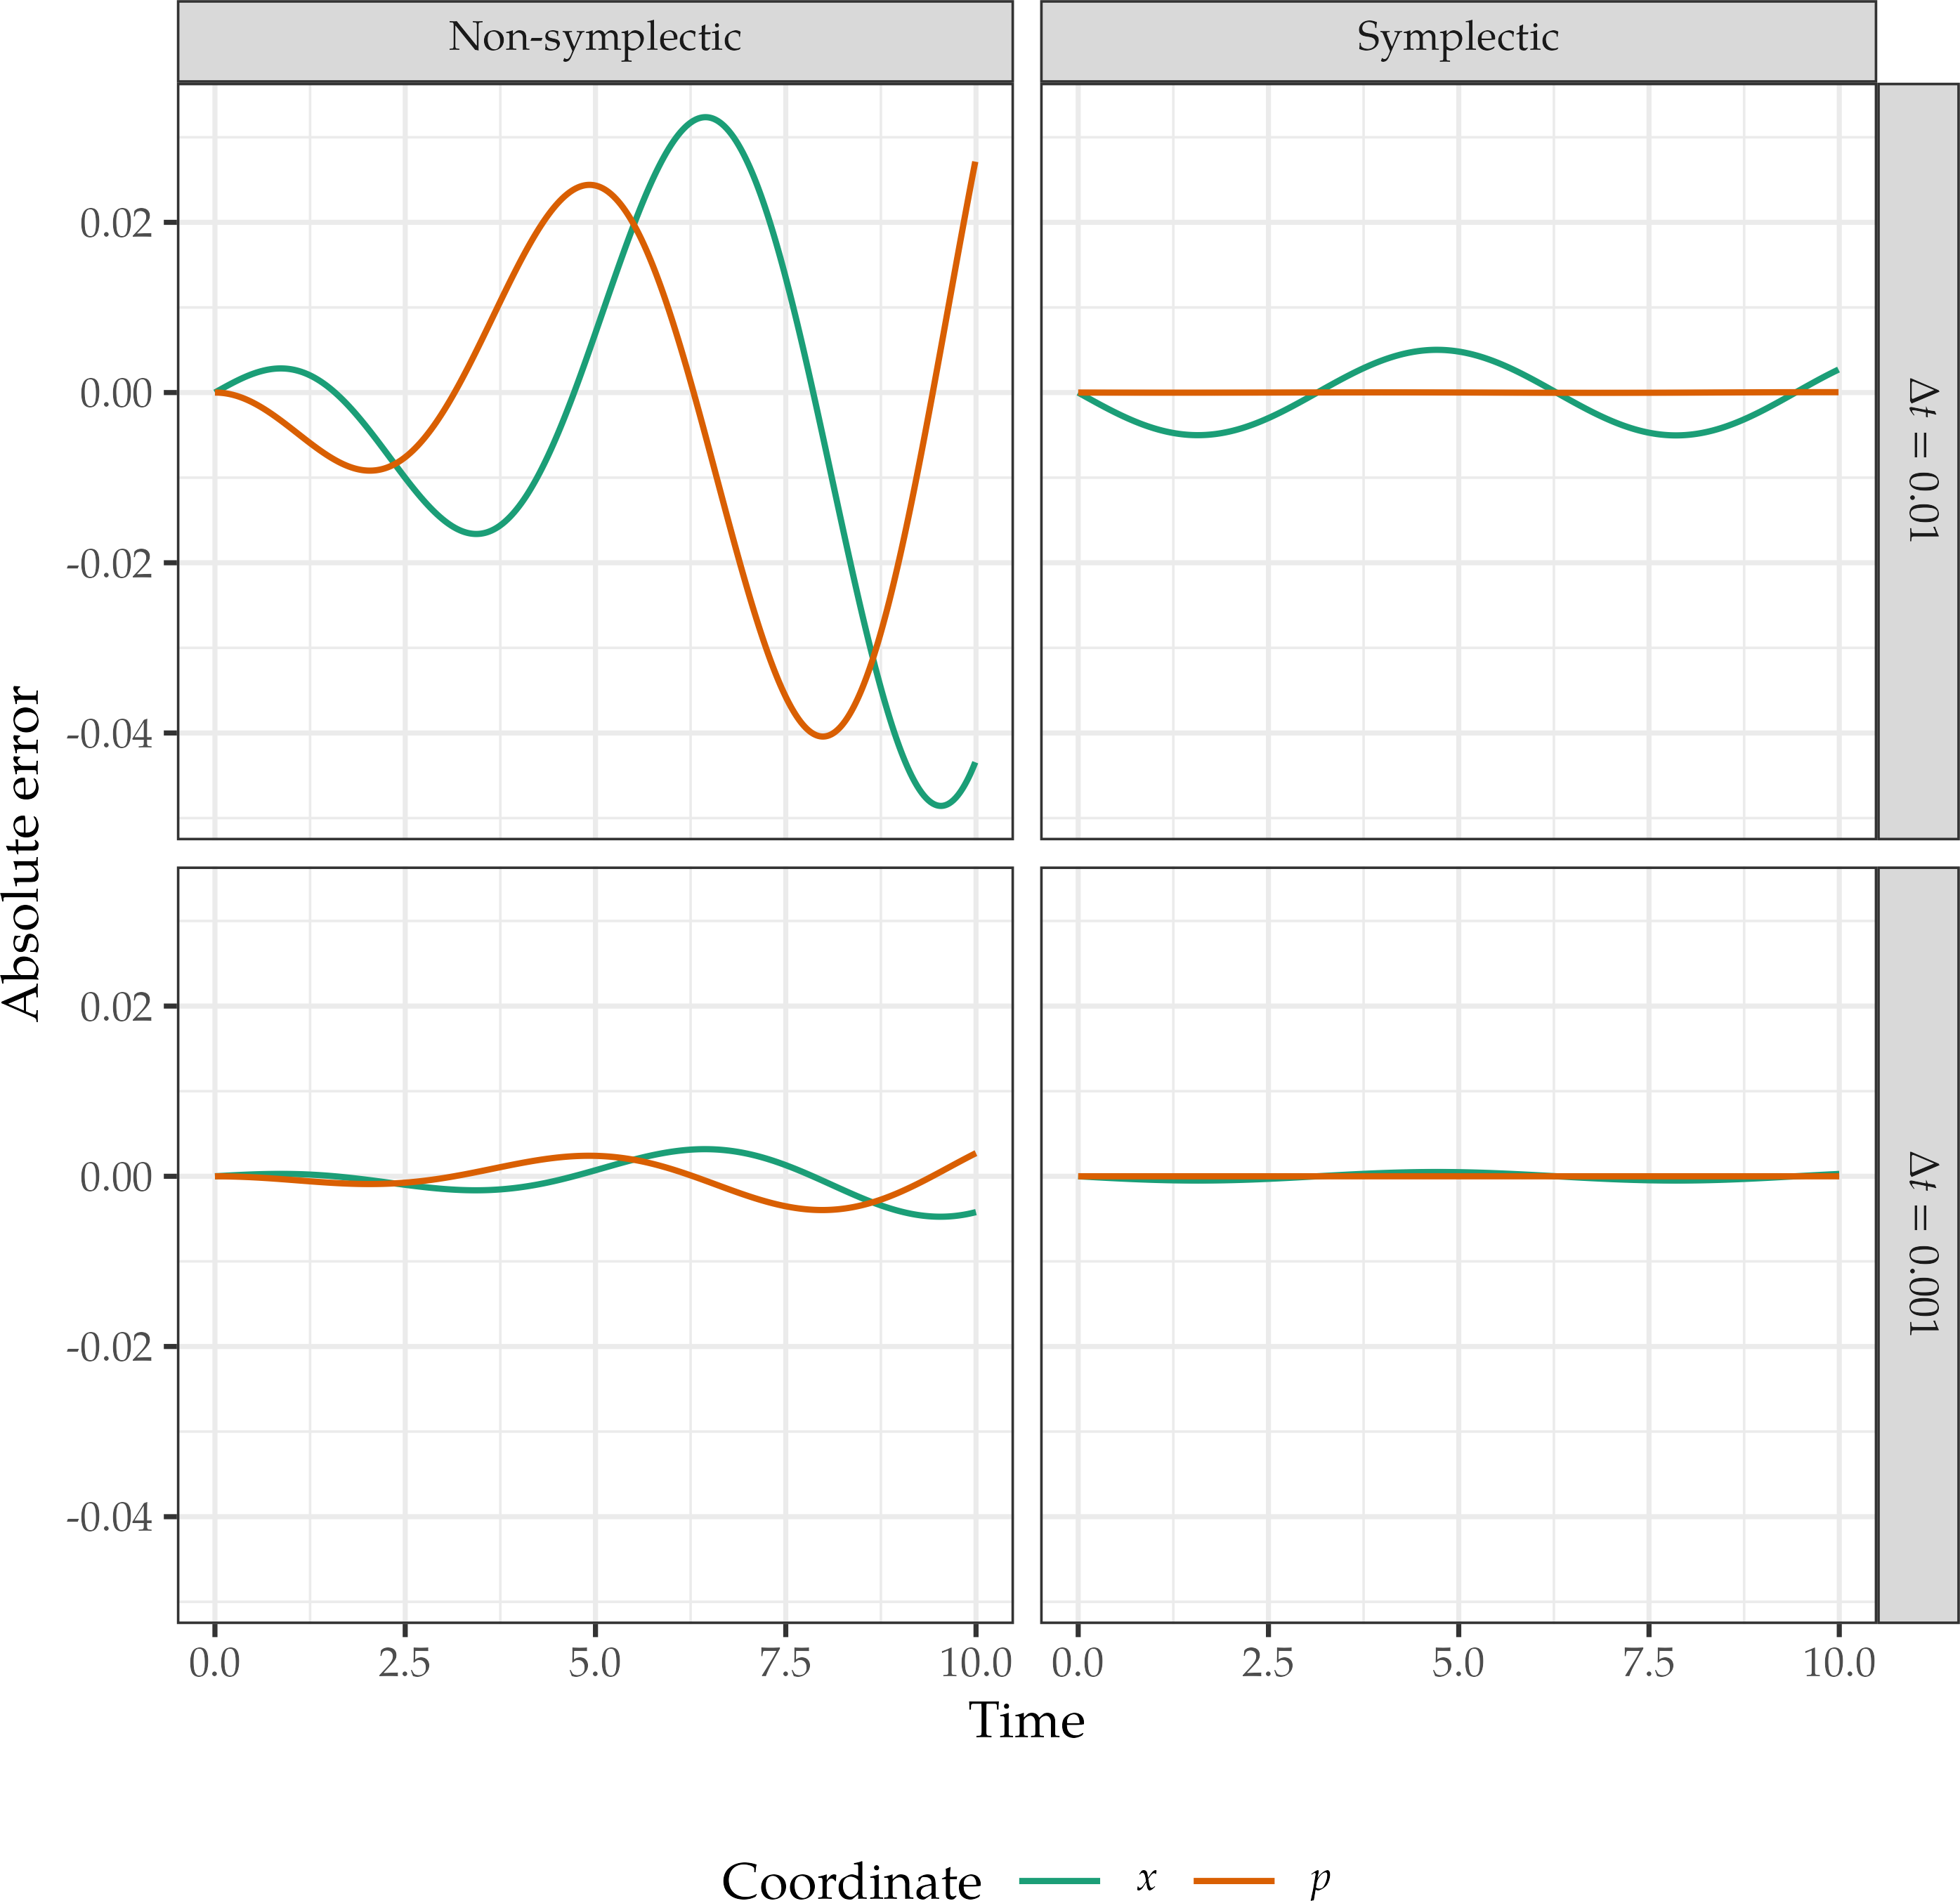
\includegraphics{img/091a}
  \caption{absolute error of $x(t)$ and $p(t)$ for the one-dimensional harmonic
    oscillator integrated with the non-symplectic integrator in
    \cref{eq:non-symp} (left panels) and the symplectic integrator in
    \cref{eq:symp} (right panels). The two upper panels refer to an integration
    with time step $\Delta t = \num{0.01}$, the bottom two to $\Delta t =
    \num{0.001}$.}
  \label{fig:091a}
\end{figure}

\Cref{fig:091a} shows the absolute integration error of the two presented
schemes compared to the exact solution $(x_{t}, p_{t}) = (\cos t, -\sin t)$
(with starting condition $x_{0} = 1$, $p_{0} = 0$) at two different time steps:
$\Delta t = \num{0.01}$ and $\Delta t = \num{0.001}$. As expected, the error is
smaller with $\Delta t = \num{0.001}$. Additionally, the symplectic integrator's
errors remain smaller and stable over time, in contrast to the non-symplectic
integrator, whose errors increase with time. \Cref{fig:091b} shows the values of
the Hamiltonian and the shadow Hamiltonian from \cref{eq:shadow-H} over time.
The symplectic integrator correctly preserves $\mathcal{H}^{\prime}$, while its
Hamiltonian displays stationary oscillations around the true value. In the case
of the non-symplectic integrator, the Hamiltonian grows linearly in time, and
$\mathcal{H}^{\prime}$ is the one that oscillates around it, also growing in
time.

\begin{figure}
  \centering
  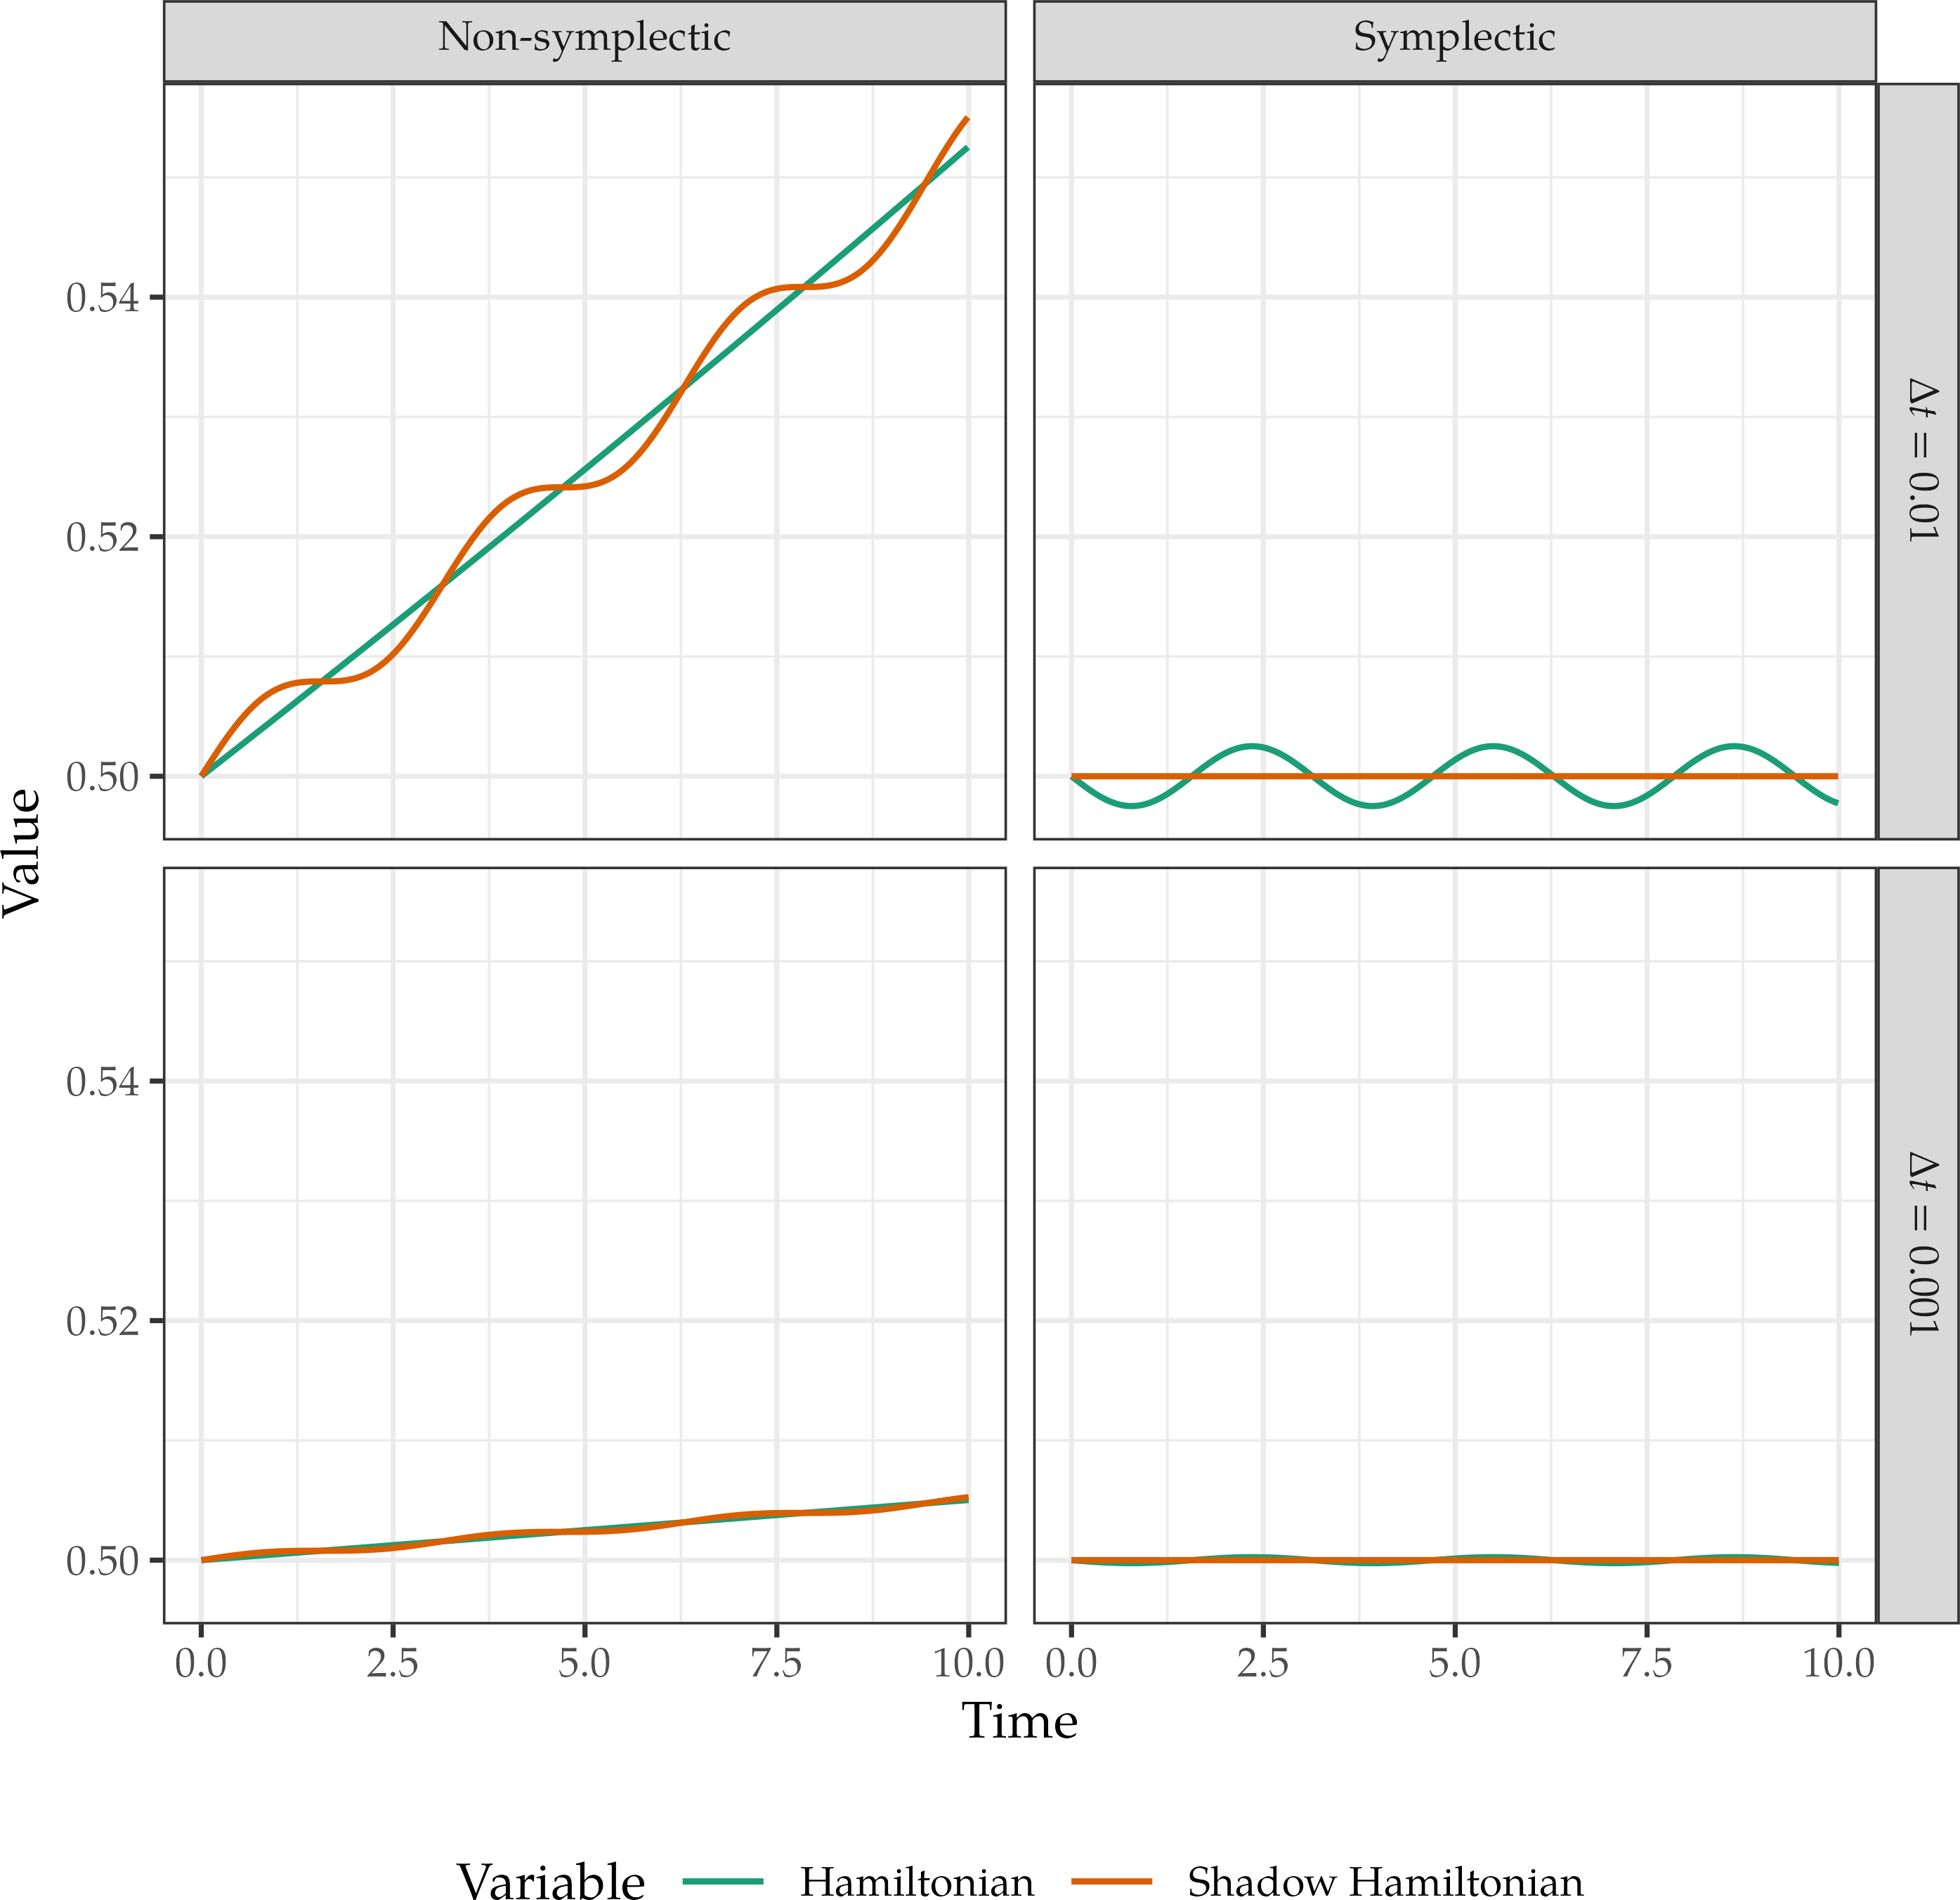
\includegraphics{img/091b}
  \caption{Hamiltonian and shadow Hamiltonian of the one-dimensional harmonic
    oscillator integrated with the non-symplectic integrator in
    \cref{eq:non-symp} (left panels) and the symplectic integrator in
    \cref{eq:symp} (right panels). The two upper panels refer to an integration
    with time step $\Delta t = \num{0.01}$, the bottom two to $\Delta t =
    \num{0.001}$.}
  \label{fig:091b}
\end{figure}
